\section{Methodology}\label{meth}
In this section, our approach to the re-implementation of the experiments will be discussed and an additional experiment will be proposed.
% Explain your approach - did you use the author's code, or did you aim to re-implement the approach ferom the description in the paper? Summarize the resources (code, documentation, GPUs) that you used.

\subsection{Code}
The code accompanying the paper is provided in \textit{C++}. As required for this study, we reproduced the work in Python, and subsequently made use of the inherent Pythonic efficiencies. The provided code allowed for a smooth initial reproduction. However, many optimisations were required to decrease computation duration.

\subsection{Model descriptions}
In the original paper, two types of single item selection models are considered: the secretary algorithm and the prophet algorithm. Candidates are partitioned into different groups which the authors refer to as \textit{colors}. Every candidate has a numerical value that indicates the capabilities of that candidate. The authors refer to these indicators as \textit{values}. Candidates arrive sequentially, and upon arrival, the algorithms decide whether the candidate is the best candidate overall. The best candidate is defined as the candidate with the highest value of the sequence of candidates. For clarity, the main parts of the Methodology and Results sections are divided per model.

\subsubsection{Secretary Algorithm}
For the secretary algorithm, it is assumed that candidates arrive in uniformly random order. To verify the claims made by the author, we compare the optimal online algorithm as proposed by \cite{correa2021fairness} to two baselines. Additionally, the algorithm and its baselines are applied on different data sets, either synthetically generated or composed from real-word data sets. The optimal online algorithm proposed by the authors (Fair secretary algorithm) is denoted formally as:
\begin{figure}[H]
    \centering
    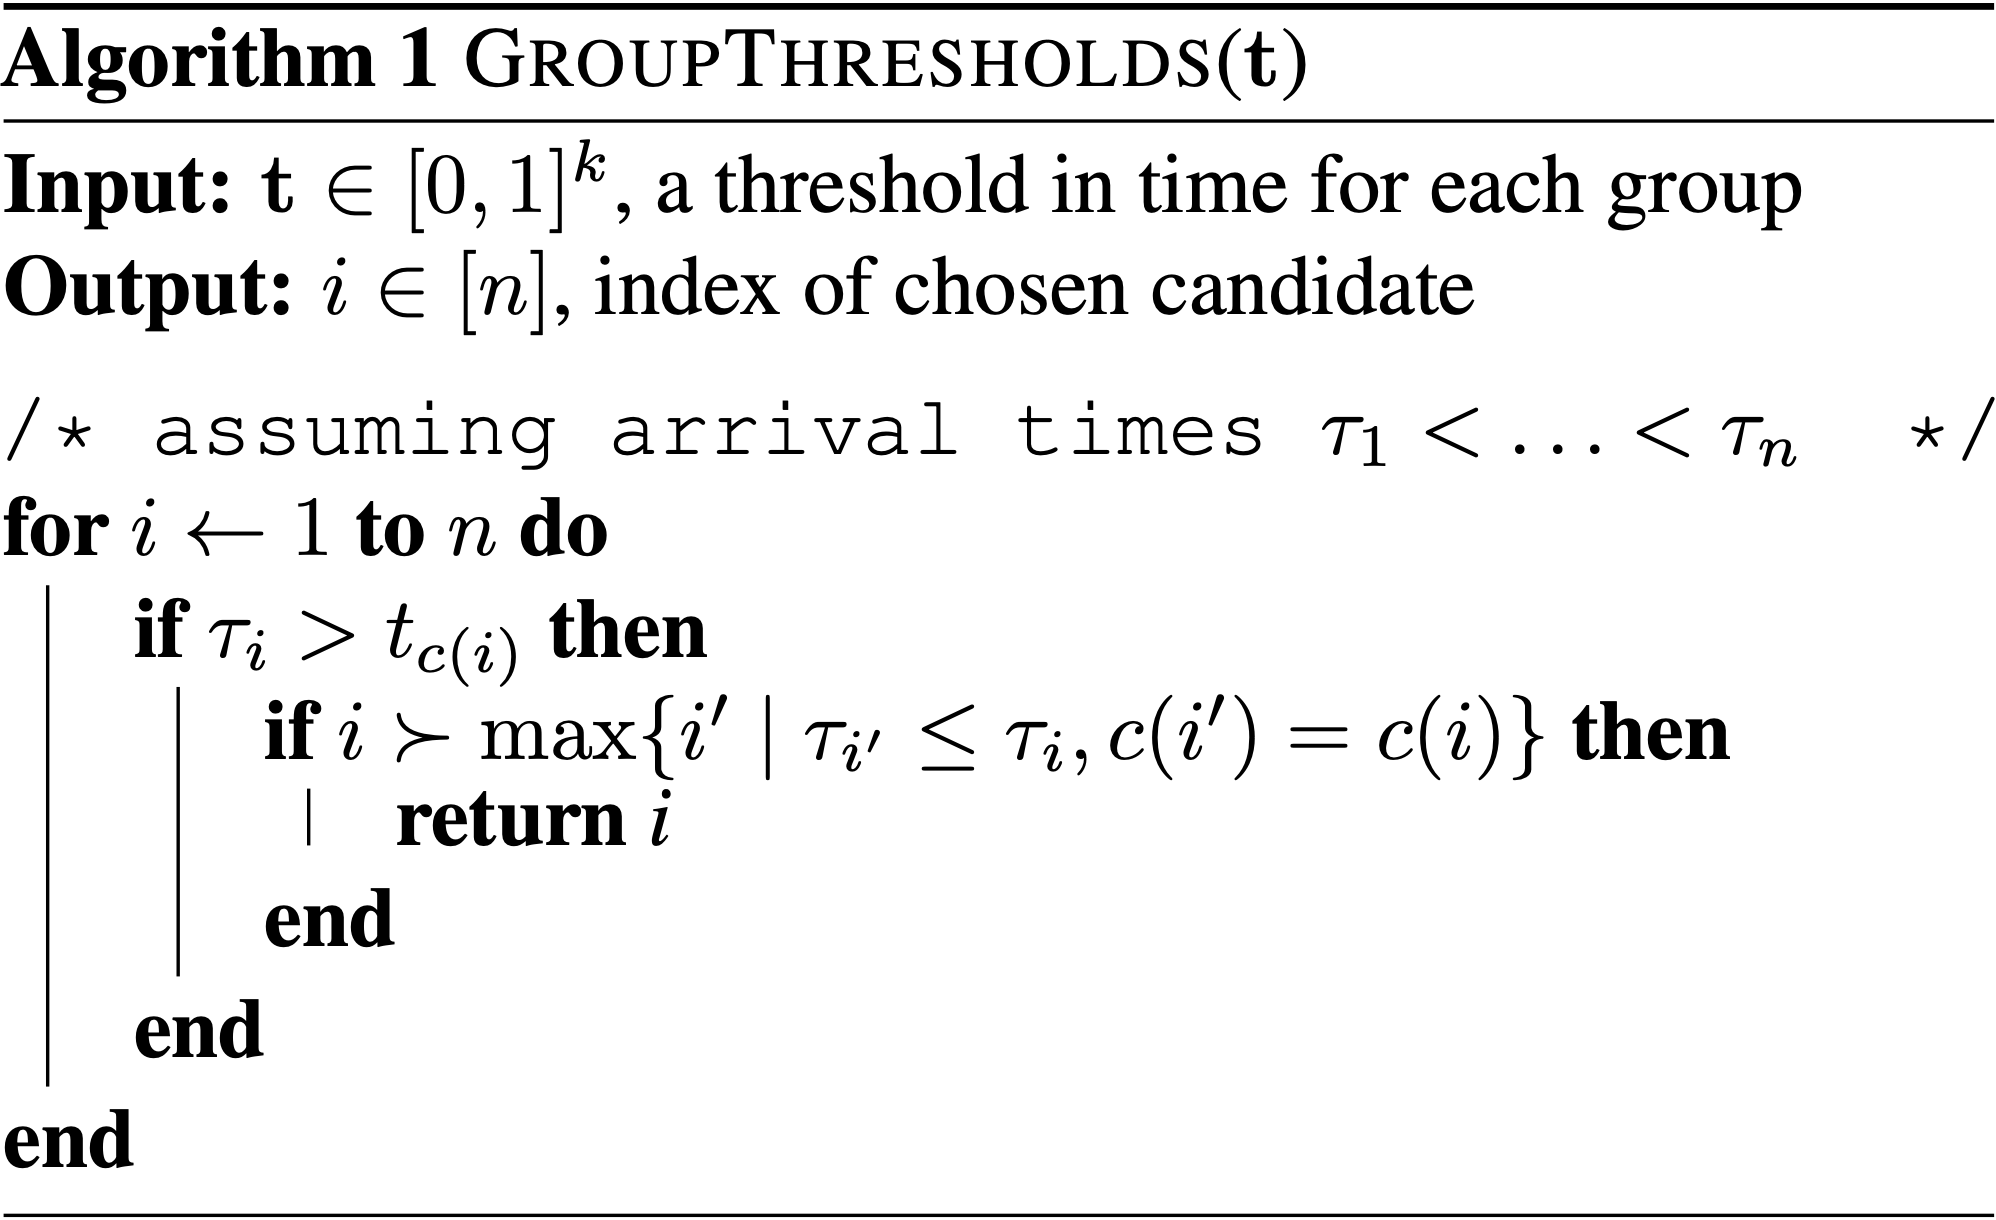
\includegraphics[width=0.5\linewidth]{media/algosa.png}
    \label{fig:algosa}
\end{figure}
% \begin{algorithm}
% \caption{GroupThresholds(t)}
% \begin{algorithmic}
% \KwInput{\mathbf{t} \in[0,1]^{k}, a threshold in time for each group}
%  \KwOutput{i \in[n], index of chosen candidate }
% \end{algorithmic}
% \end{algorithm}

where the input \textbf{t} $= (t_1, ..., t_k)$ is a vector of thresholds, one for each color $j \in [k]$. The algorithm first checks if the candidate $i$ arrived after the threshold of its color $t_{c(i)}$. If this condition is met, it accepts the candidate if its value exceeds the value of all previous candidates of color $t_{c(i)}$, indicating that it is the best candidate for that color.

After having chosen the best candidate of each color, we are interested in selecting the best overall candidate. We denote the probabilities with which the best candidate of group $j$ is the best among all colors by $p_j$, which results in the vector \textbf{p} $= (p_1,...,p_k)$ covering all colors. We use this in our experiments to verify the claims of the author using equal, and unequal values for \textbf{p} among colors.

\subsubsection{Prophet Algorithm}
For the prophet algorithm, the same assumptions are made as for the secretary algorithm, but we know the distributions $F_i$ the candidate values are drawn from. In the paper, the authors propose two optimal online algorithms specified in figure \ref{fig:prophetalgos}, where $q_1, \cdots, q_n$ denote the marginal probabilities that the optimal fair offline algorithm picks the candidates $i=1, \cdots, n$. Figure \ref{fig:genpro} shows the general Fair prophet algorithm (Fair prophet algorithm). This algorithm does not make any assumptions about the underlying probability distribution, it can be different for every candidate. Figure \ref{fig:iidpro} shows the Fair independent and identically distributed prophet algorithm (Fair IID prophet algorithm). This algorithm assumes that the values of the candidates are drawn from the same distribution.

\begin{figure*}[h!]
    \centering
    \begin{subfigure}[t!]{0.475\textwidth}
         \centering
        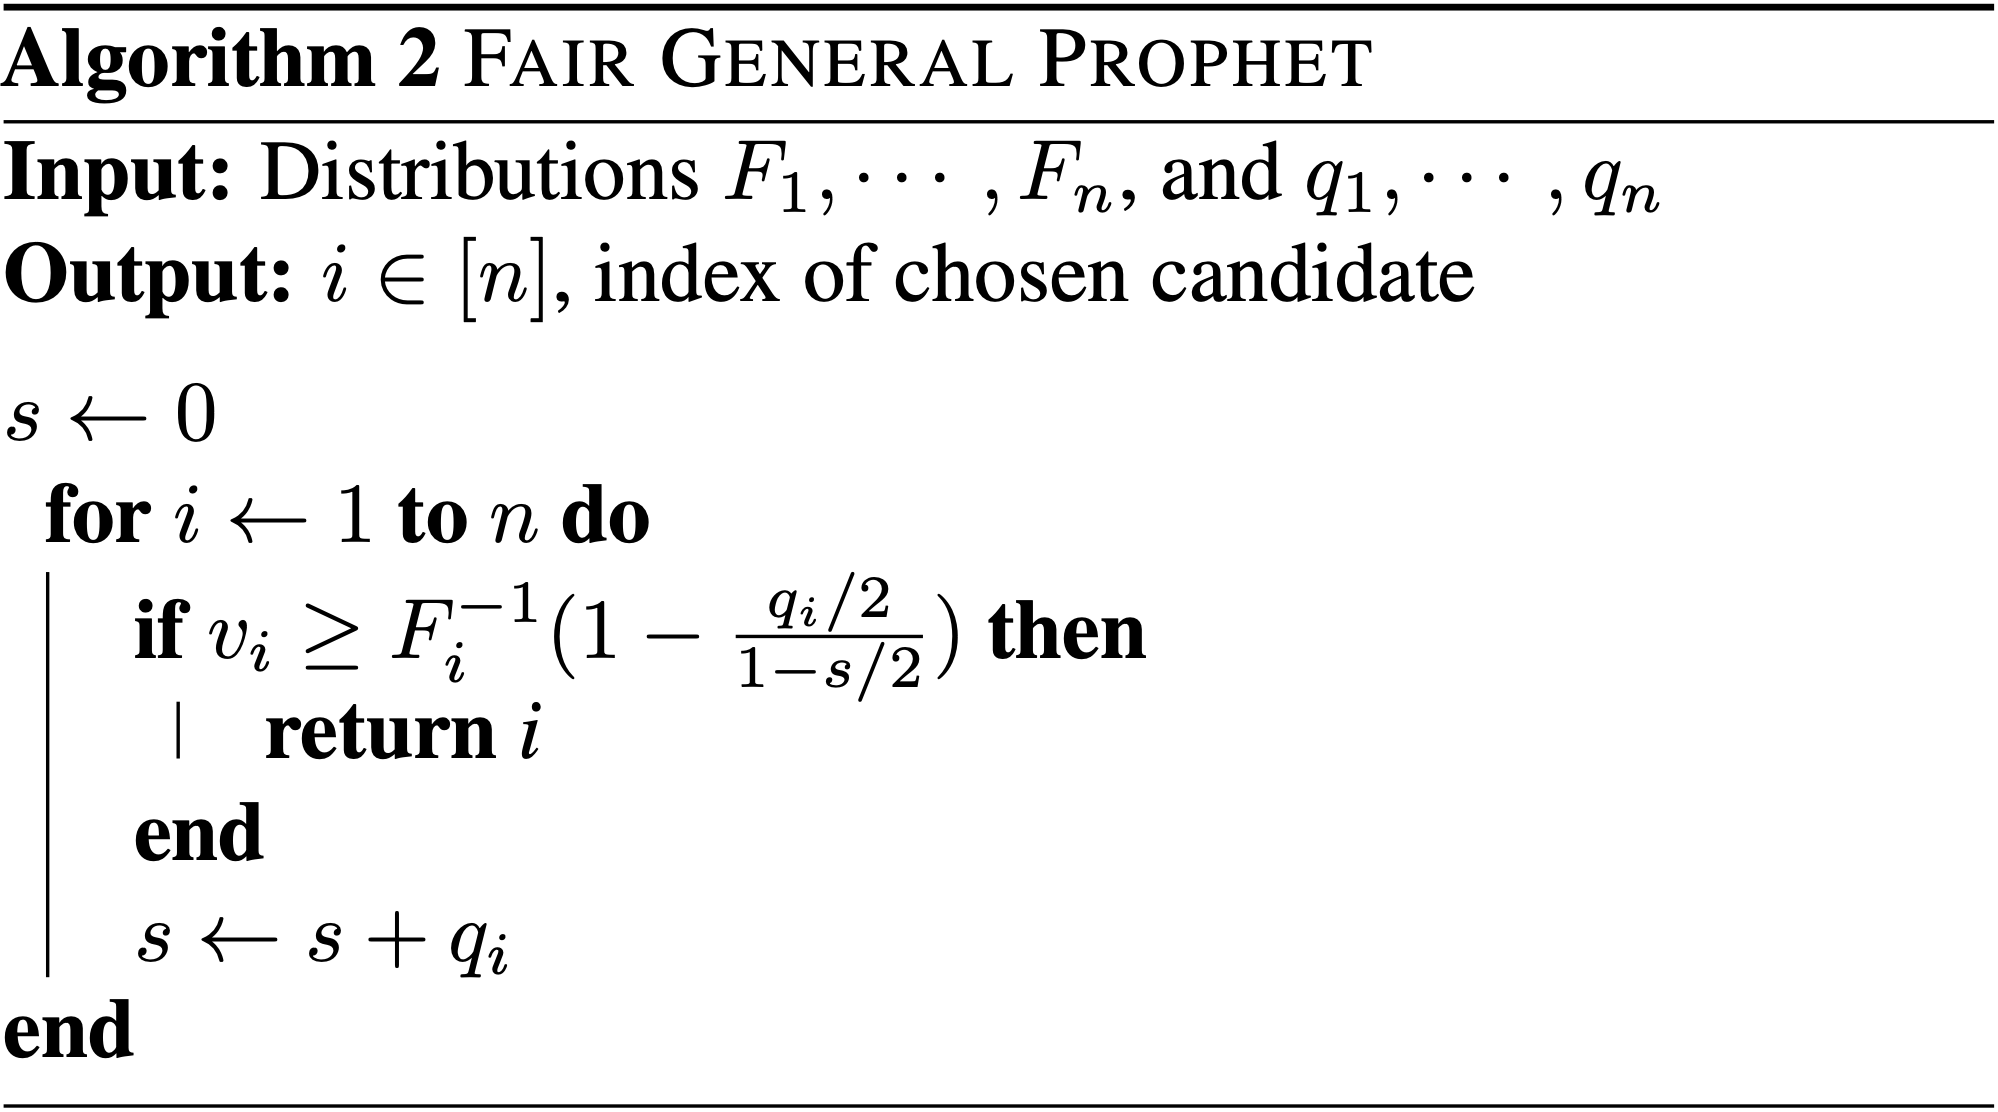
\includegraphics[width=1\textwidth]{media/generalpro.png}
        \caption{Fair prophet algorithm}
        \label{fig:genpro}
    \end{subfigure}
    \hfill
    \begin{subfigure}[t!]{0.475\textwidth}
        \centering
        \includegraphics[width=1\textwidth]{media/iddpro.png}
        \caption{Fair IID prophet algorithm}
        \label{fig:iidpro}
    \end{subfigure}
    \caption{Fair prophet algorithms proposed by the authors.}
    \label{fig:prophetalgos}
\end{figure*}

% Include a description of each model or algorithm used. Be sure to list the type of model, the number of parameters, and other relevant info (e.g. if it's pretrained).

\subsection{Data sets}
% For each data set include 1) relevant statistics such as the number of examples and label distributions, 2) details of train / dev / test splits, 3) an explanation of any preprocessing done, and 4) a link to download the data (if available).
The experiments involving the SA algorithm are conducted on two synthetic data sets and two real-world data sets. The data sets and their properties are summarised below:

\begin{enumerate}
    \item \textbf{Synthetic data set, equal p values} contains four different colors with 10, 100, 1000, and 10000 occurrences. The value of each element is chosen independently and uniformly at random from [0, 1]. \label{equalp}
    \item \textbf{Synthetic data set, general p values} contains a similar setup as \ref{equalp}, but with \textit{p} $= (0.3, 0.25, 0.25, 0.2)$.
    \item \textbf{Feedback maximization (Bank)} contains records of direct marketing campaigns (phone calls) by a Portuguese banking institution \citep{bankport}. The clients are split into 5 colors by age: under 30, 31-40, 41-50, 51-60, and over 61 years old. The value of every client is the duration of the phone call. Moreover, an equal \textit{p} of 0.2 was used for all colors.

    \item \textbf{Influence maximization (Pokec)} contains records of the influence of users of the Pokec social network \citep{pokec}. We pre-process the data by dividing the users into 5 different colors according to their body mass index (BMI): under weighted (BMI < 18.5), normal (18.5 <= BMI < 25), over weighted (25.0 <= BMI < 30.0), obese type 1 (30.0 <= BMI < 35), and obese type 2 (BMI >= 35.0). The value is computed as the number of the followers for each user. Again, an equal \textit{p} of 0.2 was used for all colors.
    \end{enumerate}

\subsection{Experimental setup}
\label{experimental_setup}
% Include a description of how the experiments were set up that's clear enough a reader could replicate the setup.
% Include a description of the specific measure used to evaluate the experiments (e.g. accuracy, precision@K, BLEU score, etc.).
% Provide a link to your code.
In this subsection, the experimental evaluation performed by the authors is discussed. As before, a distinction between the two problems is made for clarity. Additionally, an extra experiment will be considered where the secretary algorithm will be evaluated on another real-world data set. \\
\newpage
\textbf{Secretary experiments}
\FloatBarrier
\label{Secretary_Experiments}
The authors propose two different baselines to compare the Fair secretary algorithm to. Firstly, the classic secretary algorithm (SA), which does not take the colors of the candidates into account. Secondly, the single-color secretary algorithm (SCSA). This algorithm picks a color proportional to the \textit{p} values and then runs the classic secretary algorithm on the candidates of only that color. To evaluate the claims by the authors, the three mentioned algorithms are evaluated against the four data sets discussed earlier.

The parameters of these experiments consist of the size of the data sets and the number of repetitions. For the experiments on the Synthetic data sets (equal \textit{p} / general \textit{p}) and the Bank data set, all available candidates were used in 20.000 repetitions. In the original paper, the authors used all $\pm$ 650.000 candidates of the Pokec data set in 1000.000 repetitions. In our experiment, we had to limit these parameters due to time constraints. We only considered the first 40.000 candidates and used 40.000 repetitions.\\

% \newpage
\textbf{Prophet experiments}
\FloatBarrier
\label{Prophet_Experiments}
For the prophet experiments, the Fair prophet algorithm and Fair IID prophet algorithm are evaluated against three baselines: the SC algorithm \citep{samuel1984comparison}, EHKS algorithm \citep{marx2021proceedings}, CFHOV algorithm \citep{correa2021posted} and DP algorithm \citep{brown1972great}. The specific works of these algorithms are described in further detail in the paper \citep{correa2021fairness} section 4.2.

For the experiments, two settings are implemented. In the first setting, 50 samples are taken from a uniform distribution in a range of [0, 1]. These samples function as the input stream. In the second setting, 1000 samples are taken from a binomial distribution with 1000 trials and a probability of a successful single trial $p = 0.5$. In order to compare this method with the already existing algorithms, we assume each candidate to be group of its own. For every algorithm, we repeat the experiment 50.000 times.\\

\textbf{Extending to other data set (UFRGS) experiments}
\FloatBarrier
\label{Work_beyond_original_paper}
This subsection describes an experimental extension on the work of \cite{correa2021fairness}. In our work, we have concluded that the secretary results claimed in the paper are reproducible. It is shown in section \ref{results_reproducting_original_paper} that the Fair algorithm significantly outperforms the SCSA baseline. However, all real-world data sets used to prove this claim contain the same distribution of values for every color. The distributions for the Bank and Pokec data sets are shown in Figures \ref{distribution_bank} \ref{distribution_pokec} respectively.

Our extension investigates the effect of applying the Fair algorithm to an unequally distributed real-word data set, such as the UFRGS Entrance Exam and GPA Data (UFRGS) data set. This work will show whether the claims made by the authors generalize to these types of data sets. The UFRGS contains entrance exam scores of students applying to a university in Brazil (Federal University of Rio Grande do Sul), along with the students' GPAs during the first three semesters at university. The data set also includes the gender of every student (male or female).
The distribution of the data set is shown in Figure \ref{distribution_ufrgs}. This experiment is a duplication of the original secretary experiments but with the UFRGS data set as input. The gender of the students is used as color, their GPA score as values. The experiment is repeated 20.000 times.

\begin{figure*}[h!]
    \centering
    \begin{subfigure}[t]{0.32\textwidth}
         \centering
        \includegraphics[width=1\textwidth]{media/Images_plots/dataset_distribution_Bank.png}
        \caption{Bank data set}
        \label{distribution_bank}
    \end{subfigure}
    \hfill
    \begin{subfigure}[t]{0.32\textwidth}
        \centering
        \includegraphics[width=1\textwidth]{media/Images_plots/dataset_distribution_Pokec.png}
        \caption{Pokec data set}
        \label{distribution_pokec}
    \end{subfigure}
    \begin{subfigure}[t]{0.32\textwidth}
        \centering
        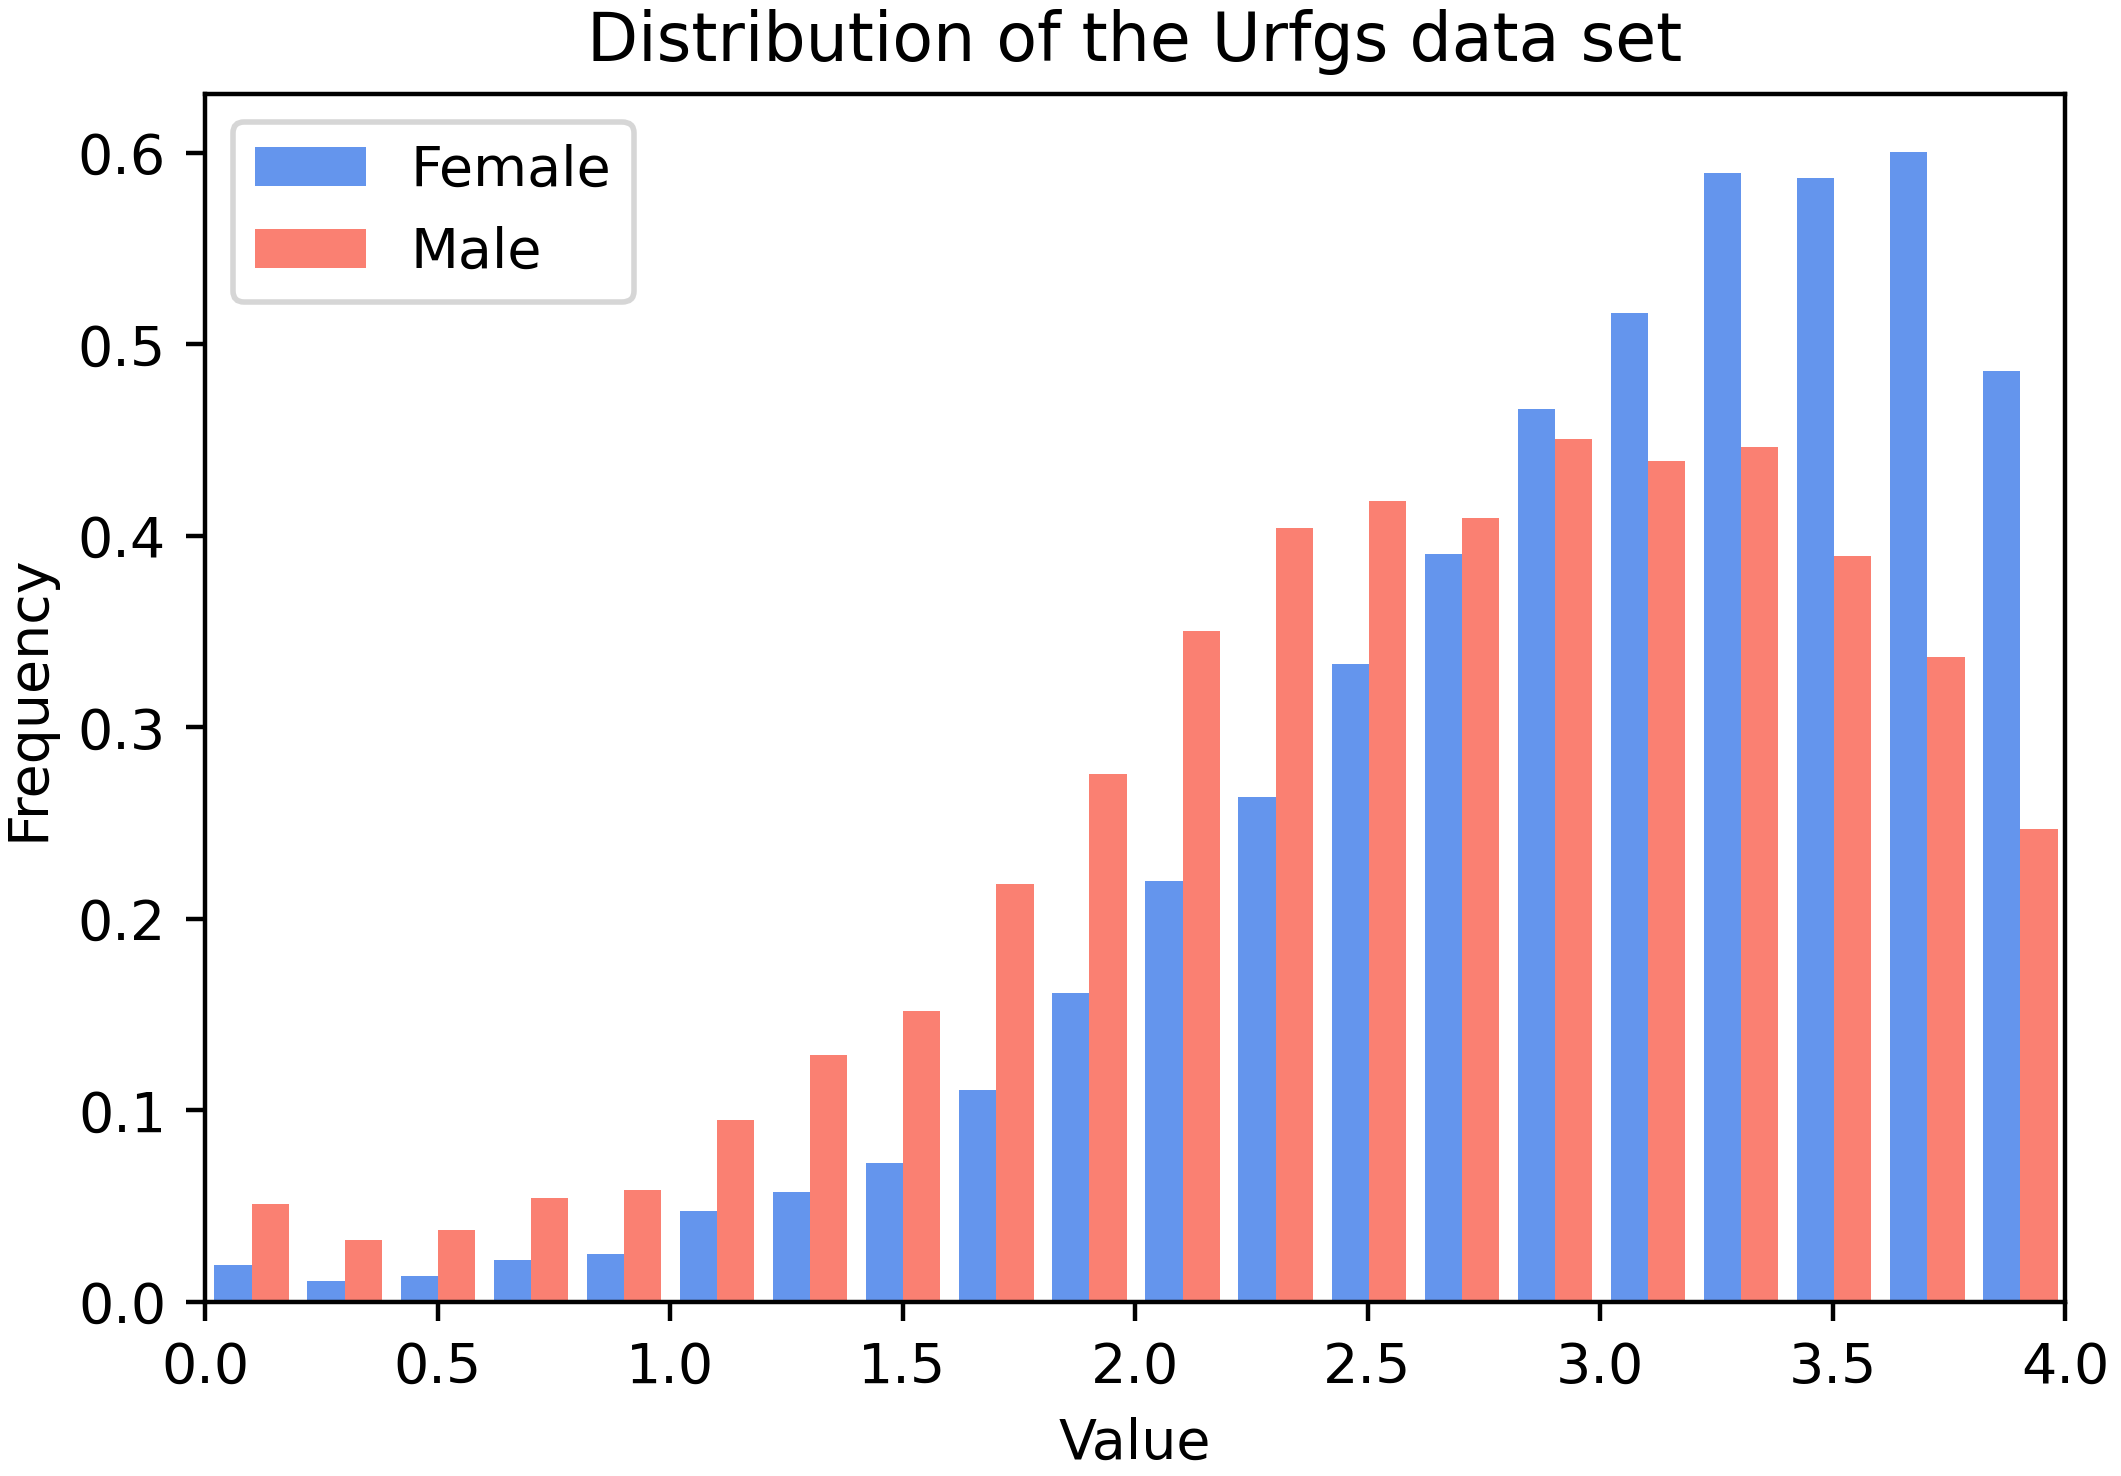
\includegraphics[width=1\textwidth]{media/Images_plots/dataset_distribution_Urfgs.png}
        \caption{Urfgs data set}
        \label{distribution_ufrgs}
    \end{subfigure}
    \caption{Value distributions of the different color groups in the real-world secretary algorithm data sets.}
    \label{fig:distributions}
\end{figure*}

% \subsection{Computational requirements}
% Include a description of the hardware used, such as the GPU or CPU the experiments were run on.
% For each model, include a measure of the average runtime (e.g. average time to predict labels for a given validation set with a particular batch size).
% For each experiment, include the total computational requirements (e.g. the total GPU hours spent).
% (Note: you'll likely have to record this as you run your experiments, so it's better to think about it ahead of time). Generally, consider the perspective of a reader who wants to use the approach described in the paper --- list what they would find useful.
% , , , 
